To evaluate the accuracy of each classification method, the system inferred possible actions with inputs from a pre-recoded test set. The test set was constructed with one member of the research team moving the arm around in an predetermined sequence that covers all the different actions. The actions at each time step is then labeled by the same member of the research team and set as the ground truth. We then feed the test data into the system and compared the inferred action with the ground truth. Following is the table that shows the accuracy of each classification method.
\begin{center}
\begin{tabular}{|l|c|c|c|r|}
\hline
Method & Total & Correct & Error & Accuracy\\ \hline
K Nearest Neighbors & 1437 & 735 & 702 & 0.511482 \\ \hline
Logistic Regression & 1437 & 1220 & 217 & 0.848991 \\ \hline
SVM(Linear Kernel) & 1437 & 1075 & 362 & 0.748086 \\ \hline
\end{tabular}
\end{center}
Besides total accuracy, we also plotted out the comparison between ground truth and inferred action over all time step for each classification method.
\begin{figure}[H]
  \centering
    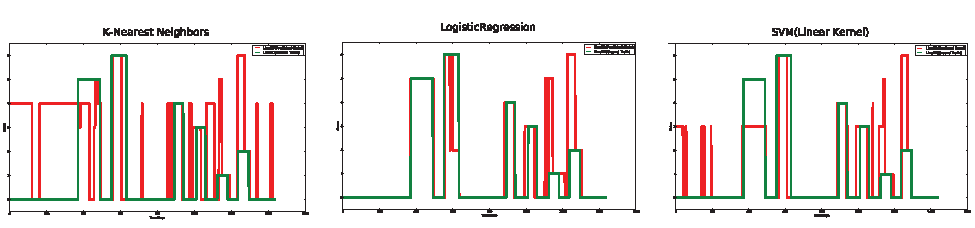
\includegraphics[width=\textwidth]{graph2}
  \caption{From left to right:KNN, Logistic Regression, SVM}
  \label{fig:sys}
\end{figure}
The y axis is different types of action inferred by the system. The lowest point, 0 is the resting position(user did not move the hand). From bottom to up are forward, backward, left, right, upward and downward.

\section{Discussion and Limitations}
From the results , we observe that KNN performed the worst. One possible reason is that the training samples for action 4(the most common false positive) spans a larger feature space and overlap with over actions. This would have confused the system and often categorizing the action for that action. The next best forming classification is SVM. We hypothesized that SVM would perform the best and did not expect it to be outperform by Logistic Regression. Again looking at the data, the SVM had a false positive for action 3 more than others. SVM might have similar issues as KNN where their margin overlaps with others. Logistic Regression performed the best in our test set and also being the only classifier that was able to at some point classify all action correctly. However, there still are multiple false positive that needed to be address in future iterations. From a usability standpoint, the system might benefit more from having more false negatives instead of false positive since it will be more frustrating if the system misunderstood you compare to it doing nothing.
